\documentclass{vgtc}                          % final (conference style)
\usepackage[utf8]{inputenc}
\usepackage[T1]{fontenc}
%\documentclass[review]{vgtc}                 % review
%\documentclass[widereview]{vgtc}             % wide-spaced review
%\documentclass[preprint]{vgtc}               % preprint
%\documentclass[electronic]{vgtc}             % electronic version
\usepackage{graphicx}                % allow us to embed graphics files
\DeclareGraphicsExtensions{.pdf,.png,.jpg,.jpeg} % for pdflatex we expect .pdf, .png, or .jpg files
%% it is recomended to use ``\autoref{sec:bla}'' instead of ``Fig.~\ref{sec:bla}''
\graphicspath{{figures/}{pictures/}{images/}{./}} % where to search for the images

\usepackage{hyperref}

\usepackage{microtype}                 % use micro-typography (slightly more compact, better to read)
\PassOptionsToPackage{warn}{textcomp}  % to address font issues with \textrightarrow
\usepackage{textcomp}                  % use better special symbols
\usepackage{mathptmx}                  % use matching math font
\usepackage{times}                     % we use Times as the main font
\renewcommand*\ttdefault{txtt}         % a nicer typewriter font
\usepackage{cite}                      % needed to automatically sort the references
\usepackage{tabu}                      % only used for the table example
\usepackage{booktabs}                  % only used for the table example

%% In preprint mode you may define your own headline.
%\preprinttext{To appear in an IEEE VGTC sponsored conference.}

%% Paper title.

\title{Visualizing Bayesian Optimization for Teaching}

\author{William M. Temple\thanks{e-mail: William.Temple@colorado.edu}\\ %
        \scriptsize University of Colorado Boulder
}%


%% Abstract section.
\abstract{Effectively teaching machine learning, with its high cognitive load,
demands exceptional teaching utilities. Often, students find abstract
discussions or overly-formal mathematical discriptions either difficult to
interpret and understand or insufficiently applicable. In this article, I
explore the application of data visualization techniques to Bayesian
Optimization (Gaussian Processes) and describe the tasks that students engaged
in hypothetical study of this model would likely perform. We further develop
some prototype user-interfaces and address technological challenges essential
to the development of an interactive system for studying Bayesian
Optimization.} % end of abstract

%%%%%%%%%%%%%%%%%%%%%%%%%%%%%%%%%%%%%%%%%%%%%%%%%%%%%%%%%%%%%%%%
%%%%%%%%%%%%%%%%%%%%%% START OF THE PAPER %%%%%%%%%%%%%%%%%%%%%%
%%%%%%%%%%%%%%%%%%%%%%%%%%%%%%%%%%%%%%%%%%%%%%%%%%%%%%%%%%%%%%%%%

\begin{document}

\firstsection{Introduction}

\maketitle

Educational technology systems present interesting design challenges when
analyzed using a data-visualization lens.  Students have different goals
and desires and separate motivations from data analysts. For better or
worse, much of the discourse about data visualization in our coursework
and in the literature we have read for class has focused on the consumption
of data by analysts---or, at least, by users (even untrained or novice users)
\textit{performing} an analytical role.

However, as we have a broad interest in the development of educational tools for
novice Computer Science and Programming students, we always try to consider the
ways in which the data visualization techniques that we have discussed apply in
the classroom to enhance the educational experience and provide for a more
robust pedagogy.

Towards this goal, in this project we have focused on building a tool to analyze
the state of a machine learning algorithm. In particular, the system shows the
execution of a Bayesian Optimization using a Gaussian Process Regression. The
system allows a curious user to examine the state of the model and shows not
merely the \textit{result} of the application of the model (which would be the
primary interest of users in analytical roles), but also makes evident the
choices that the model makes during execution and empowers the user to
understand the mathematical reasoning behind those choices.

\subsection{Why Gaussian Processes?}

The Guassian Process is an advanced stochastic process which uses a suite of
functions and strategies for optimizing those functions to create estimations
of the mean and variance over a distribution of other functions\footnote{Prof.
Nando de Freitas's video lecture at the University of British Columbia on the
subject of Gaussian Processes contains the requisite background
knowledge~\cite{nando}}. That is to say, it is relatively complicated.

However, a computer can execute Bayesian Optimization in a small series of abstract steps:

\begin{enumerate}

	\item Initialize the Algorithm by sampling a small number of random
		points from a true function $f$ and fitting an initial
		regression using a \textit{kernel} function.

	\item Use an \textit{acquisition} function to choose a point which is
		likely to improve the estimated mean of the process.

	\item Sample that point and add it to the regression.

	\item Repeat until the model converges on an accurate estimation of
		$f$.

\end{enumerate}

That is to say, the Gaussian Process isn't so complicated that it evades an
effective decomposition through visualization. It also has certain essential
properties that we believe make it particularly suited to a visual approach to
teaching its concepts. We discuss these properties further in Section 3.

\section{Related Work}

In this section, we discuss some existing literature which informs our design
choices and our thinking about how visualization and task modeling in particular
relate to the goal of education. We also include some discussion of existing
education literature which we feel aids our explanation of why visualization
provides an augmentation to the learning environment.

\subsection{Teaching as Presentation}

While many forms of visualization cater to analytical interests, in teaching we
wish to present information rather than analyze it. As instructors, we want to
integrate knowledge into our courses in such a way that it is ``memorable'' and
``engaging.'' Robert Kosara describes \textit{Presentation-Oriented
Visualization Techniques} in exactly those words, then he further constrains
presentation-oriented techniques: ``presentation-oriented techniques need to be
specific rather than general and compact rather than scalable''~\cite{Kosara}.
In other words, a presentation does not need to account for the countless ways
that a user may want to use it, as its primary purpose is to convey the
information that the author (or presenter) desires. In teaching, 

As teachers (presenters), we attempt to anchor information into our students'
minds. ``To get people to actually pay attention to a presentation, they need
to find the views interesting and engaging... Learnability,'' Kosara declares,
``is part of this''~\cite{Kosara}. If we take Kosara's concerns into account,
then we should aim to build a tool that (1) clearly shows the state of our
Gaussian Process, (2) does not necessarily generalize to accomodate arbitrary
inputs, but (3) sufficiently accomodates student input so that they can explore
the visualization an an engaging way.

\subsection{Task Modeling for Learning}

Both instructors and students will engage with our visualization, but both
roles have different needs and different tasks they wish to perform. The
instructor is a presenter, while the student explores the visualization to
uncover the model's inner-workings. We can use a visualization task taxonomy to
describe the ways that students will interact with our visualization.

- What tasks do students approach an educational vis with?

- What specific tasks are we going to accomodate?

\subsection{Knowledge Construction}

In Constructivist eductation paradigms, the presentation of examples is
essential to the development of accurate knowledge. Mordechai Ben-Ari describes
constructivism as ``a theory of learning, which claims that students construct
knowledge rather than merely receive and store knowledge transmitted by the
teacher''~\cite{benari}. We agree with this assessment, as such the function
of our visualization is to facilitate model-building. Ultimately the student learns
of her own accord, and our role as visualization designer is to provide a space in
which learning happens.

Several studies have attested to the efficacy of worked-examples practice, in
which students observe and attempt to understand the process that leads to the
correct answer to a proposed problem~\cite{kirschner}. Our visualization bears
similarity to worked-example practice, as it shows the process by which an
approximate estimation is derived, rather than merely its result. We believe
that this form of visualization will guide students to a correct interpretation
of Bayesian Optimization based on the effectiveness of similar example styles
that have been deployed in algebra classrooms~\cite{workex}.

\section{Design}

Due to time and resource constraints, as well as considerations about scope
listed in the Related Works section above, we decided to restrict the kinds of
functions available to the user and focus on creating a compelling
visualization for one configuration of Bayesian Optimization. The configuration
we ultimately chose utilizes the Upper Confidence Bound (UCB) acquisition
function (with a $\kappa$ parameter of 20), a Matérn kernel function (with a
$\nu$ parameter of 2.5), and a fixed true function $f(x,y)$ composed of a
linear combination of $x$ and $y$ as well as seven Gaussian Distributions (with
random means and standard-deviations).

We chose these parameters qualitatively, based on our assessment that this
configuration produced the most obvious, evident, and correspondent effects in
the display, so that we would have a higher chance of engaging the user with a
noticeable effect. Several configurations of the model do \textit{not} result
in interesting or memorable effects, so---in line with Kosara's reasoning given
above---we fix the parameters to this known-good state.

\begin{figure}
	\begin{center}
		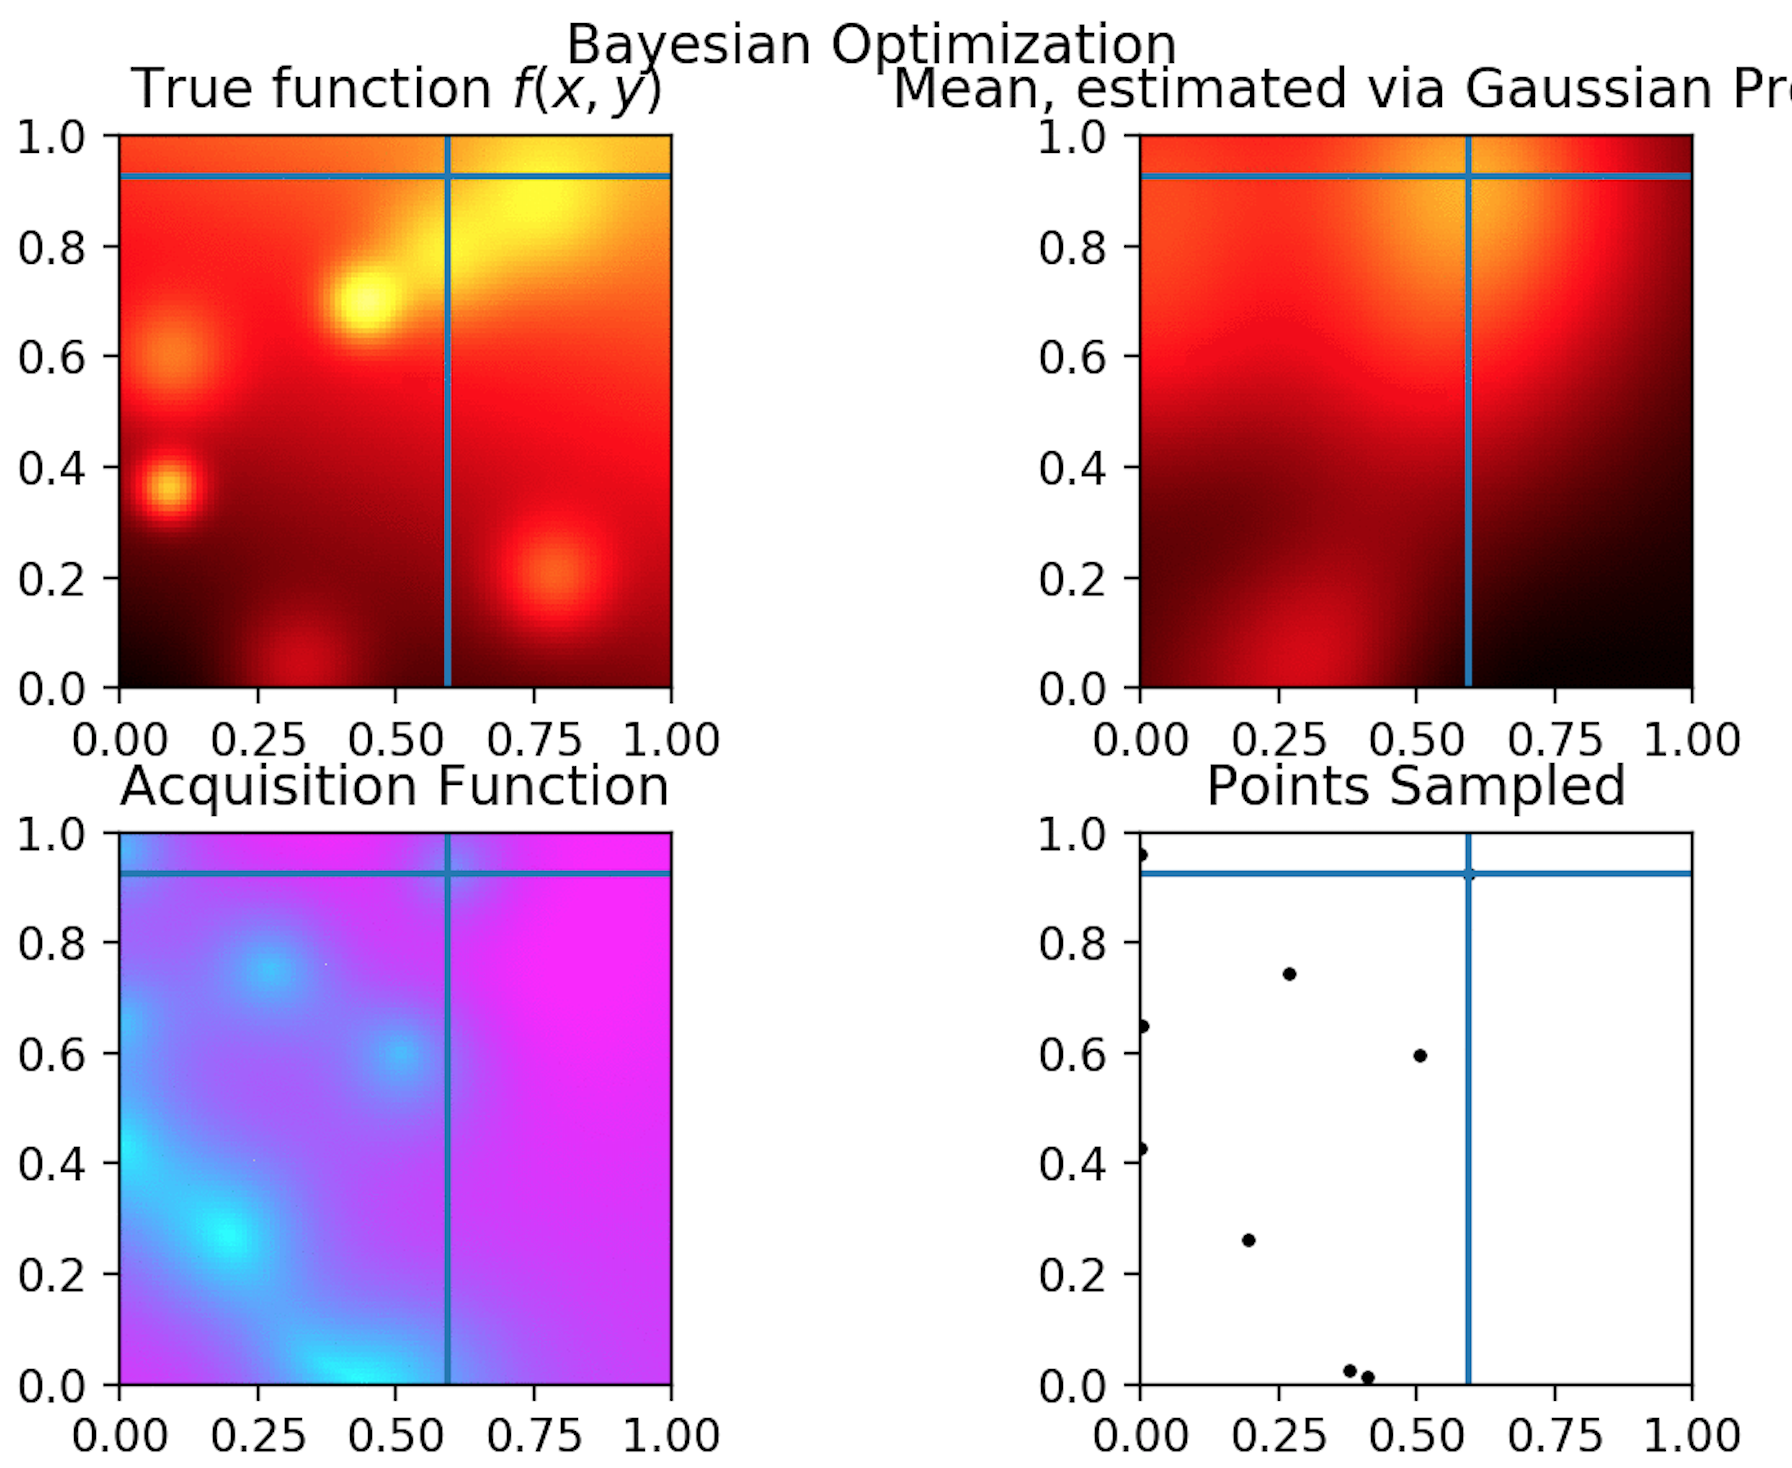
\includegraphics[width=0.4\textwidth]{fig1-full}
	\end{center}
	\caption{An example of the Python prototype interface after 9 iterations.}
	\label{f1}
\end{figure}

\subsection{User Experience}

Early in the design process, we settled on four coordinated views for the
interface. One for each of the algorithm's essential features:

\begin{itemize}

	\item \textbf{Top-Left}: a color-mapped graph showing the output of the
		true function $f(x.y)$

	\item \textbf{Top-Right}: a color-mapped graph showing the estimated
		mean of the Gaussian Process Regression

	\item \textbf{Bottom-Left}: a color-mapped graph showing the value of
		the UCB acquisition function
	
	\item \textbf{Bottom-Right}: a scatter-plot showing the set of points
		which have already been sampled and incorporated into the
		regression

\end{itemize}

The plots in our visualization are coordinated. On each iteration of the model,
they all update simultaneously to reflect the most immediate change to the
model. Each plot displays crosshairs (an intersecting vertical and horizontal
line) that denote the location of the most recent point added to the model's
regression (Figure \ref{f1}).

\subsubsection{React.js Concept UI or, Why Not Python?}

We found it very difficult to attach User-Interface elements to any
`matplotlib` elements, and in general we had little success developing a UI in
Python. This difficulty (the unsuited-ness of Python to the engineering task
of developing a rich User Interface) was a primary motivator in our decision to
pursue an alternative web-based UI. 

We developed a concept UI in React.js and Semantic UI that allowed us to
rapidly build a rich web interface. However, the web platform comes with its
own challenges. While libraries to perform Bayesian Optimization are readily
available in Python with copious tutorials and examples, on the web, we would
have to implement our own Bayesian Optimization library in JavaScript from the
ground up. In addition, due to modifications we made to use the GPU as a
coprocessor (more in the section below), we would additionally require a
GPU-friendly implementation of the Gaussian Process Regression. We believe this
is possible with a bit more effort. However, due to time and work constraints,
our project remains in two pieces: a conceptual UI with no Baysian Optimization
engine, and a Pythonic Baysian Optimizer with no user interface.

\subsection{Technical Challenges}

Early in the prototyping stages of this project, we realized that computational
complexity would pose significant challenges to the interactivity of this
software and its usability. The first Python prototypes of the software could
only compute and render one iteration of the Optimization algorithm about every
25 seconds. Through some code optimization effort, we managed to reduce the
runtime per iteration to 7 seconds, but it became clear during this process
that further optimization would require a shift in development paradigm.

At this latency, the interactivity of the system is threatened, as users may
press buttons that have no effect, and as they begin to use the software, it
takes considerably less than seven seconds to digest the information divulged
by a single iteration of the program. Rudimentary profiling of the code reveals
that the program spends the vast majority (90\%) of its time drawing the four
coordinated plots, as each plot iterates over each pixel in the its image. Even
drawing only one of the plots requires about two seconds using Python, where a
single plot consists of ten thousand points (one hundred points in both the X
and Y directions).

As a proof of concept, in order to solve this problem, we wrote GPU fragment
shader programs using the GPU.js library~\cite{GPUjs}. This library
dyanamically recompiles a restricted subset of JavaScript into GLSL shader
code, which then runs on the SIMD processors in the host machine's Graphics
Processing Unit, resulting in much faster execution. Furthermore, this shader
code deposits resulting textures directly into an HTML \texttt{<canvas>}
element, so that the browser can easily render it. We integrated these fragment
shaders into our concept UI application, and measured that the same machine
could render a function of the same complexity as those in our Python program at
several times the resolution (2048 points in both the X and Y direction) in
about 110 milliseconds~\footnote{Test machine: 6-CPU Intel i7, 16GB Memory,
NVIDIA GeForce GTX 960 Graphics Accelerator}.

\section{Discussion}

\subsection{Prototype Artifacts}

\section{Conclusion}

%\bibliographystyle{abbrv}
\bibliographystyle{abbrv-doi}
%\bibliographystyle{abbrv-doi-narrow}
%\bibliographystyle{abbrv-doi-hyperref}
%\bibliographystyle{abbrv-doi-hyperref-narrow}

\bibliography{template}
\end{document}
